\section{Leading order, two flavor pion stars}


\subsection{Equation of state}
The free energy density of two-flavor chiral perturbation theory, to leading-order and at $T = 0$, is
%
\begin{equation}
    \Eff = - f^2 \left(\bar m^2 \cos \alpha + \frac{1}{2} \mu_I^2 \sin^2 \alpha\right).
\end{equation}
%
The $\alpha$ parameter is determined by minimizing $\Eff$ for a given value of $\mu_I$,
%
\begin{equation}
    \pdv{\Eff}{\alpha} = f^2 \left(\bar m^2 - \mu_I^2 \cos \alpha\right) \sin(\alpha) = 0.
\end{equation}
%
This gives an explicit formula for $\alpha$ in terms of $\mu_I$.
As long as the chemical potential is lower than the critical value $\mu_I^c = \bar m$, the only solution to this equation is $\alpha = 0$.
As the chemical potential reaches this critical value, the system undergoes a phase transition from the vacuum phase to the \emph{pion condensate} phase.
In this new phase, the solution is
%
\begin{align}
    \label{alpha as function of mu lowest order}
    \cos \alpha = \frac{\bar m^2}{\mu_I^2}.
\end{align}
%
We introduce a dimensionless variable $x^2 = \cos\alpha = \bar m^2 / \mu_I^2$.
This variable has the domain $[0, 1]$.
By an argument using a right triangle, we can verify that $\cos \alpha = x^2$ implies that $\sin^2 \alpha = 1 - x^4$.
Substituting the dimensionless variable into the free energy density, we get 
%
\begin{equation}
    \Eff = - \frac{u_0}{2} \left( x^2 + \frac{1}{x^2} \right).
\end{equation}
%
We have introduced the characteristic energy density $u_0 = \bar m^2 f^2$.
As we found in \autoref{section: cold fermi star}, the pressure is given by negative the free energy density, normalized to $\mu_I = \bar m$, or $x = 1$.
We choose $p_0 = u_0$, so the dimensionless pressure is
%
\begin{equation}
    \label{pressure leading order chpt}
    \tilde p = -\frac{1}{p_0} \left(\Eff - \Eff_{x=1}\right) 
    = \frac{1}{2} \left( x^2 + \frac{1}{x^2} - 2 \right).
\end{equation}
%
The charge density corresponding to a chemical potential is given by minus the derivative of the free energy with respect to that chemical potential. 
We must, however, not assume any dependence of $\alpha$ on $\mu_I$ when taking this derivative.
The isospin density therefore is
%
\begin{equation}
    n_I = -\pdv{\Eff}{\mu_I} = ^2 \mu_I^2 \sin^2 \alpha 
    = 
    \frac{u_0}{\mu_I} \left(\frac{1}{x^2} - x^2\right).
\end{equation}
%
With this, the dimensionless energy density at $T = 0$ is
%
\begin{equation}
    \label{energy density leading order chpt}
    \tilde u = - \tilde p + \frac{\mu_I n_I}{u_0}
    = \frac{1}{2} \left( 2 + \frac{1}{x^2} - 3 x^2\right).
\end{equation}
% 
The ratio of pressure to energy density is
%
\begin{equation} 
    \label{pressure energy ratio leading order chpt}
    \frac{p}{u} = \frac{1- 2x^2 + x^4  }{1 + 2x^2 -3x^4 }.
\end{equation}
%
In the ultrarelativistic limit, where $\mu_I \rightarrow \infty$ and thus $x \rightarrow 0$, we get $p / u = 1$, or $u_\text{ur} = p$.
In the non-relativisitc limit, that is $x^{-2} = 1 + \epsilon$, $\epsilon \ll 1$, we get $\tilde p = \epsilon^2 / 2 $, and $\tilde u = 2\epsilon$, so the equation of state is $\tilde u_\text{nr} = 2 \sqrt 2 \sqrt{\tilde p}$.
\autoref{fig: equation of state pions} shows the equation of state in two different regimes and compares it with the ultrarelativistic and non-relativistic limit.

\begin{figure}[h]
    \centering
    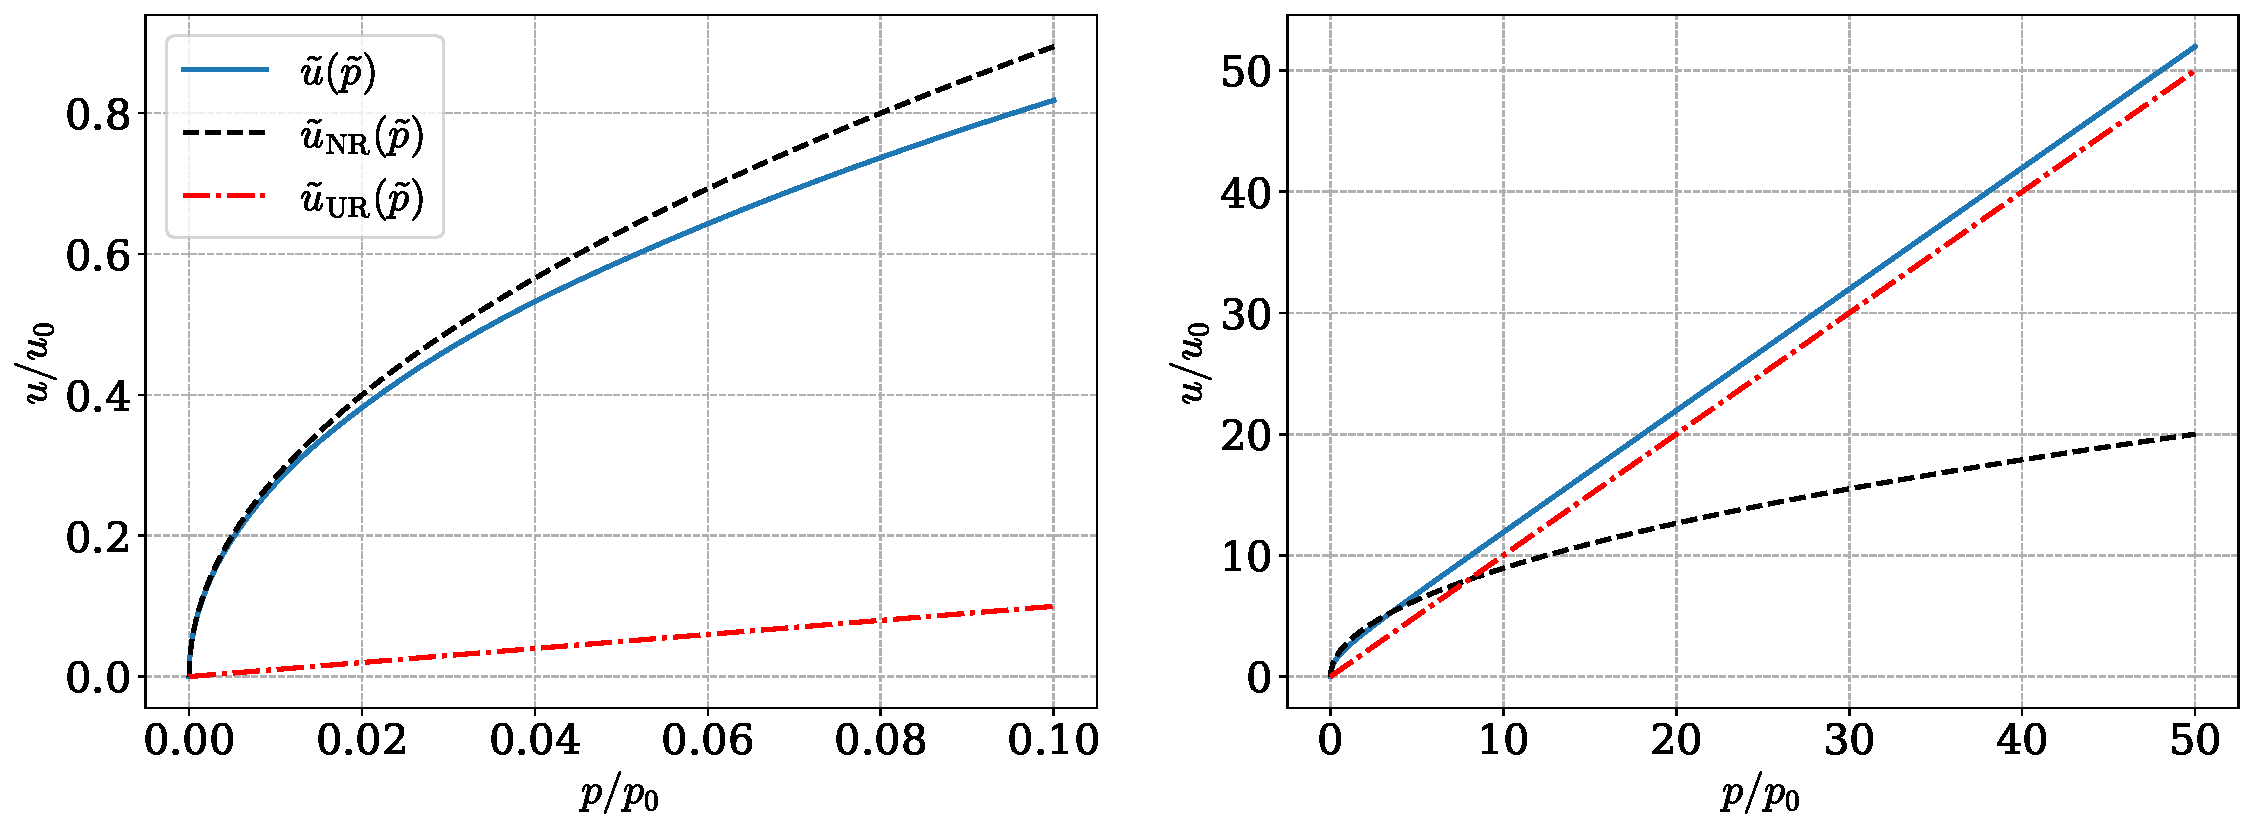
\includegraphics[width=0.95\textwidth]{../scripts/figurer/pion_star/pion_eos.pdf}
    \caption{
        This plot shows the leading order equation of state of two-flavor chiral perturbation theory and compares it with the ultrarelativistic and non-relativistic limit, shown as dashed lines. The $x$-axis shows the pressure normalized to $p_0$, while the $y$-axis shows the energy density normalized to $u_0$.
    }
    \label{fig: equation of state pions}
\end{figure}


\subsection{Units}

The characteristic mass and length, as discussed in \autoref{section: TOV equation}, are found by setting $k_1 = k_2 = k_3 = 1$.
These are the dimensionless constants of the TOV equation, \autoref{dimensionless constants TOV}.
At tree-level, the bare constants $f$ and $\bar m$ are related to physical constants by $f = f_\pi$ and $m = m_\pi$, the pion decay constant and the pion mass.
Using the values for $f_\pi$ and $m_\pi$ as given in \autoref{section: units} and reinstating $c$ and $\hbar$, these quantities are give in by
%
\begin{align}
    u_0 & =m_\pi^2 f_\pi^2 \frac{c}{\hbar^3}
    = 3.216\cdot 10^{33} \, \text{J}\,\text{m}^{-3}, \\
    m_0 & = \frac{c^4}{\sqrt{\frac{4 \pi}{ 3} u_0 G^3}} = 64.21\, M_\odot, \\
    r_0 & = \frac{G}{c^2} m_0 = 94.79 \, \text{km}.
\end{align}
%
We, therefore, expect both the radius and mass of the pion star to be around one order of magnitude larger than the star made up of cold neutrons.

\subsection{Limiting radius}

We found that the non-relativisitc limit of the equation of state is $\tilde p = 2^{-3} \tilde u^2$, i.e., it is a polytrope with $\gamma = 2$.
As discussed in \autoref{subsection: Newtonian limit and polytropes}, this corresponds to a situation where the radius of the star is independent of the central pressure, at least in the Newtonian limit of gravity.
When simulating the Newtonian, non-relativistic limit of the pion star, we should expect the radius to be constant.
From \autoref{Radius polytrope}, the radius is $R = r_0 C \xi_1$, where $\xi_1$ is the first zero of the Lane-Emden equation with $n = 1$, and
%
\begin{equation}
    C = \frac{1}{\sqrt{4(4\pi ) G u_0}} = \frac{1}{\sqrt{12}}r_0.
\end{equation}
%
To find $\xi_1$, we must find the root of
%
\begin{equation}
    \theta'' + \frac{2}{\xi} \theta' + \theta = 0.
\end{equation}
%
By substituting $\theta$ for its power series expansion, $\theta = \sum_n a_n \theta^n$, we get
%
\begin{equation}
    \sum_n \left[ (n+2)(n+1) a_{n+2} + 2(n+1) a_{n+1} \xi^{-1} + a_n \right] \xi^n = 0,
\end{equation}
%
and we get the recursion relation $a_{n+2} = - a_n / (n+1)(n+2)$.
With our boundary condition, the solution is
%
\begin{equation}
    \theta(\xi) = \frac{\sin(\xi)}{\xi},
\end{equation}
%
and the first root is therefore $\xi_1 = \pi$.
With this, we get a closed-form expression for the stellar radius of this non-relativistic and Newtonian limit---which we expect the full theory to approach as the central pressure decreases---namely
%
\begin{equation}
    \label{radius pion star nr limit}
    R = \frac{\pi}{\sqrt{12}} r_0 = 85.97 \, \text{km}.
\end{equation}


\subsection{Results}

The code used for obtaining numerical results is discussed in \autoref{appendix: code}.

\autoref{fig: pressure and mass for pion star} show the pressure and mass as a function of radius for varying values of central pressure.
The quantities are normalized to the stellar radius, stellar mass, and central pressure, respectively.
The black dashed line corresponds to the configuration with the maximum mass.
We see that both the pressure and mass distribution are very similar for stars with a mass less than the maximum.
As the central pressure increase beyond that of the star with maximum mass, the pressure gradient close to the center grows sharply.
This is similar to what we saw in the case of an incompressible fluid, \autoref{subsection: incompressible fluid}.

\begin{figure}[!h]
    \centering
    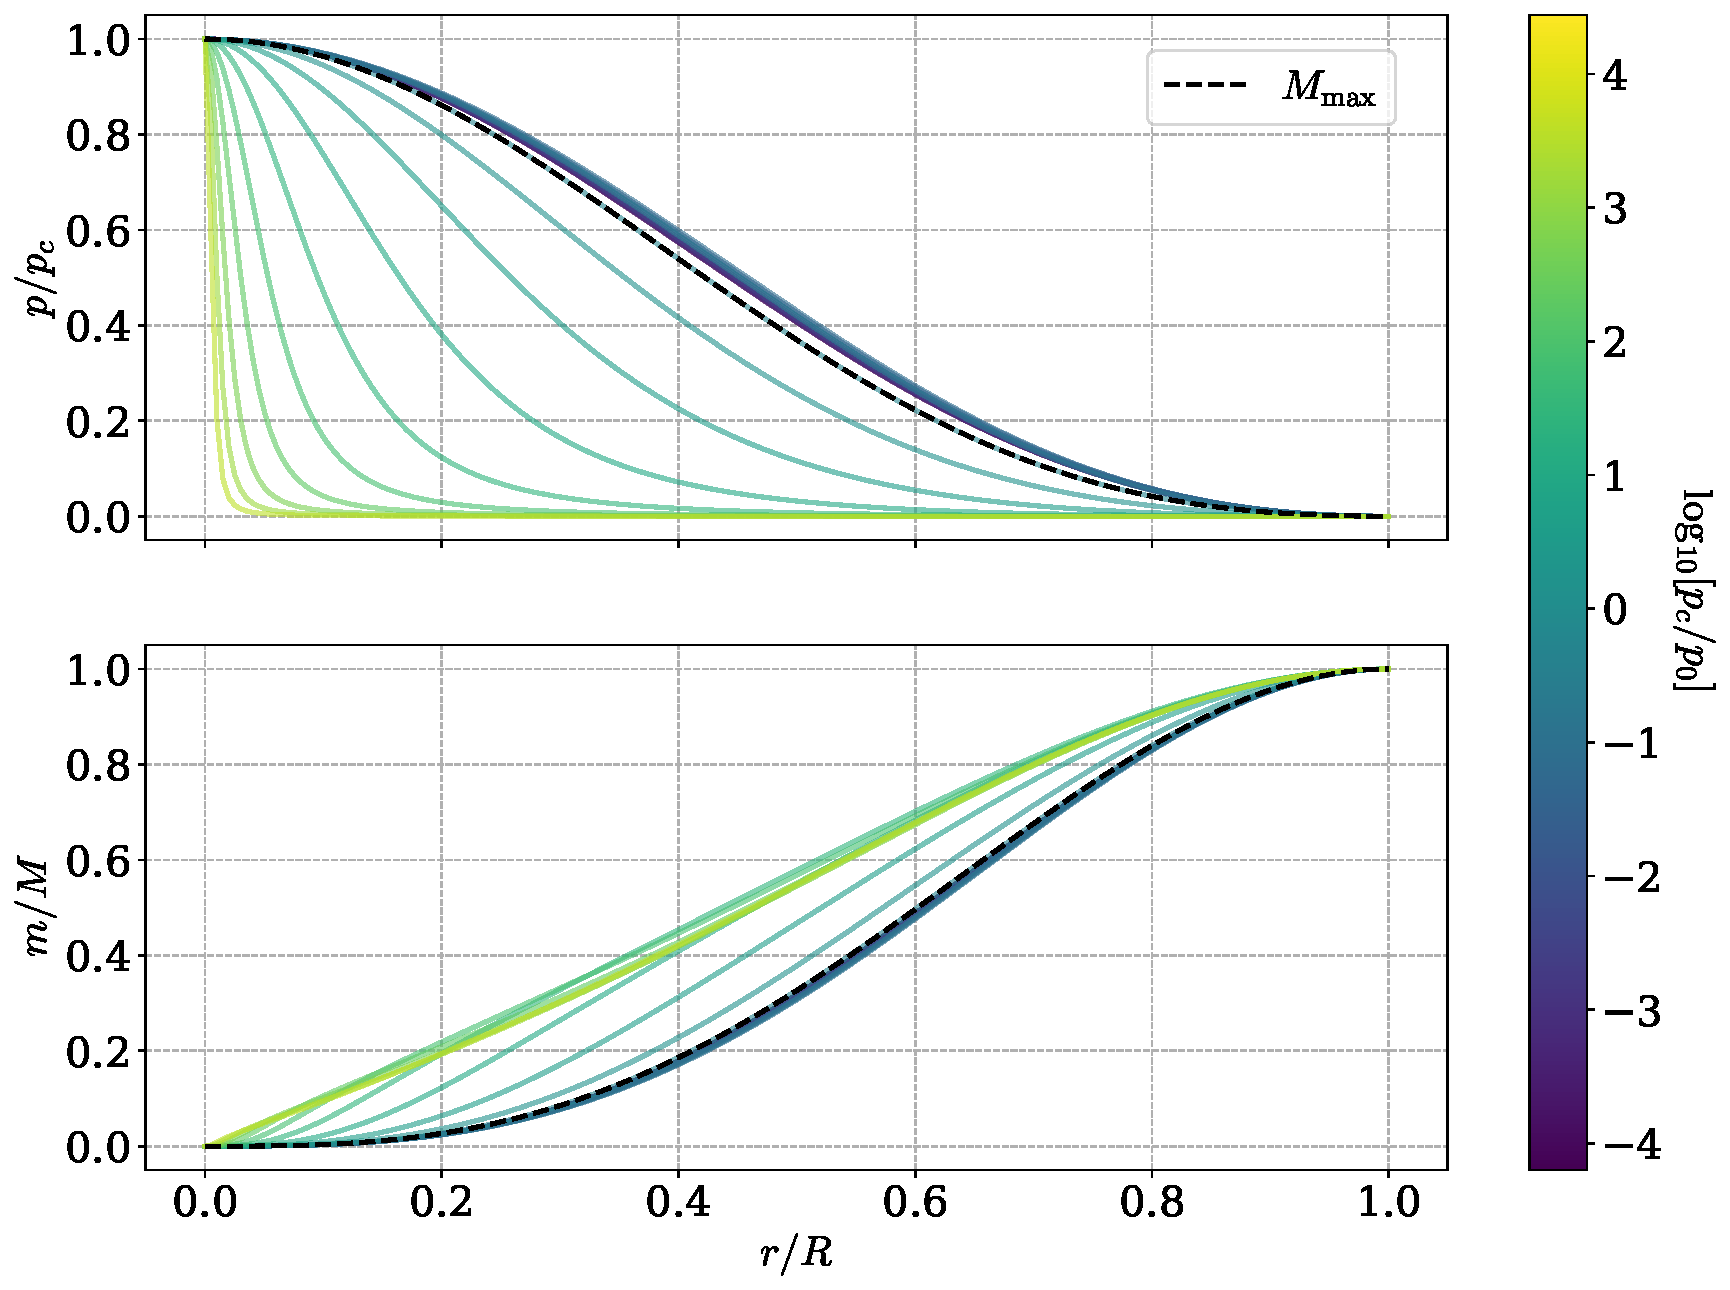
\includegraphics[width=0.8\textwidth]{../scripts/figurer/pion_star/pressure_mass_pion_star.pdf}
    \caption{
        Top: The pressure normalized to the central pressure, as a function of radius, normalized to the stellar radius.
    Bottom: The mass, normalized to stellar mass, within a radius $r$, normalized to the stellar radius.
    Both plots show a range of stars with different central pressures, indicated by the color.
    The black dashed line corresponds to the star with the largest mass.
    }
    \label{fig: pressure and mass for pion star}
\end{figure}

\begin{figure}[!h]
    \centering
    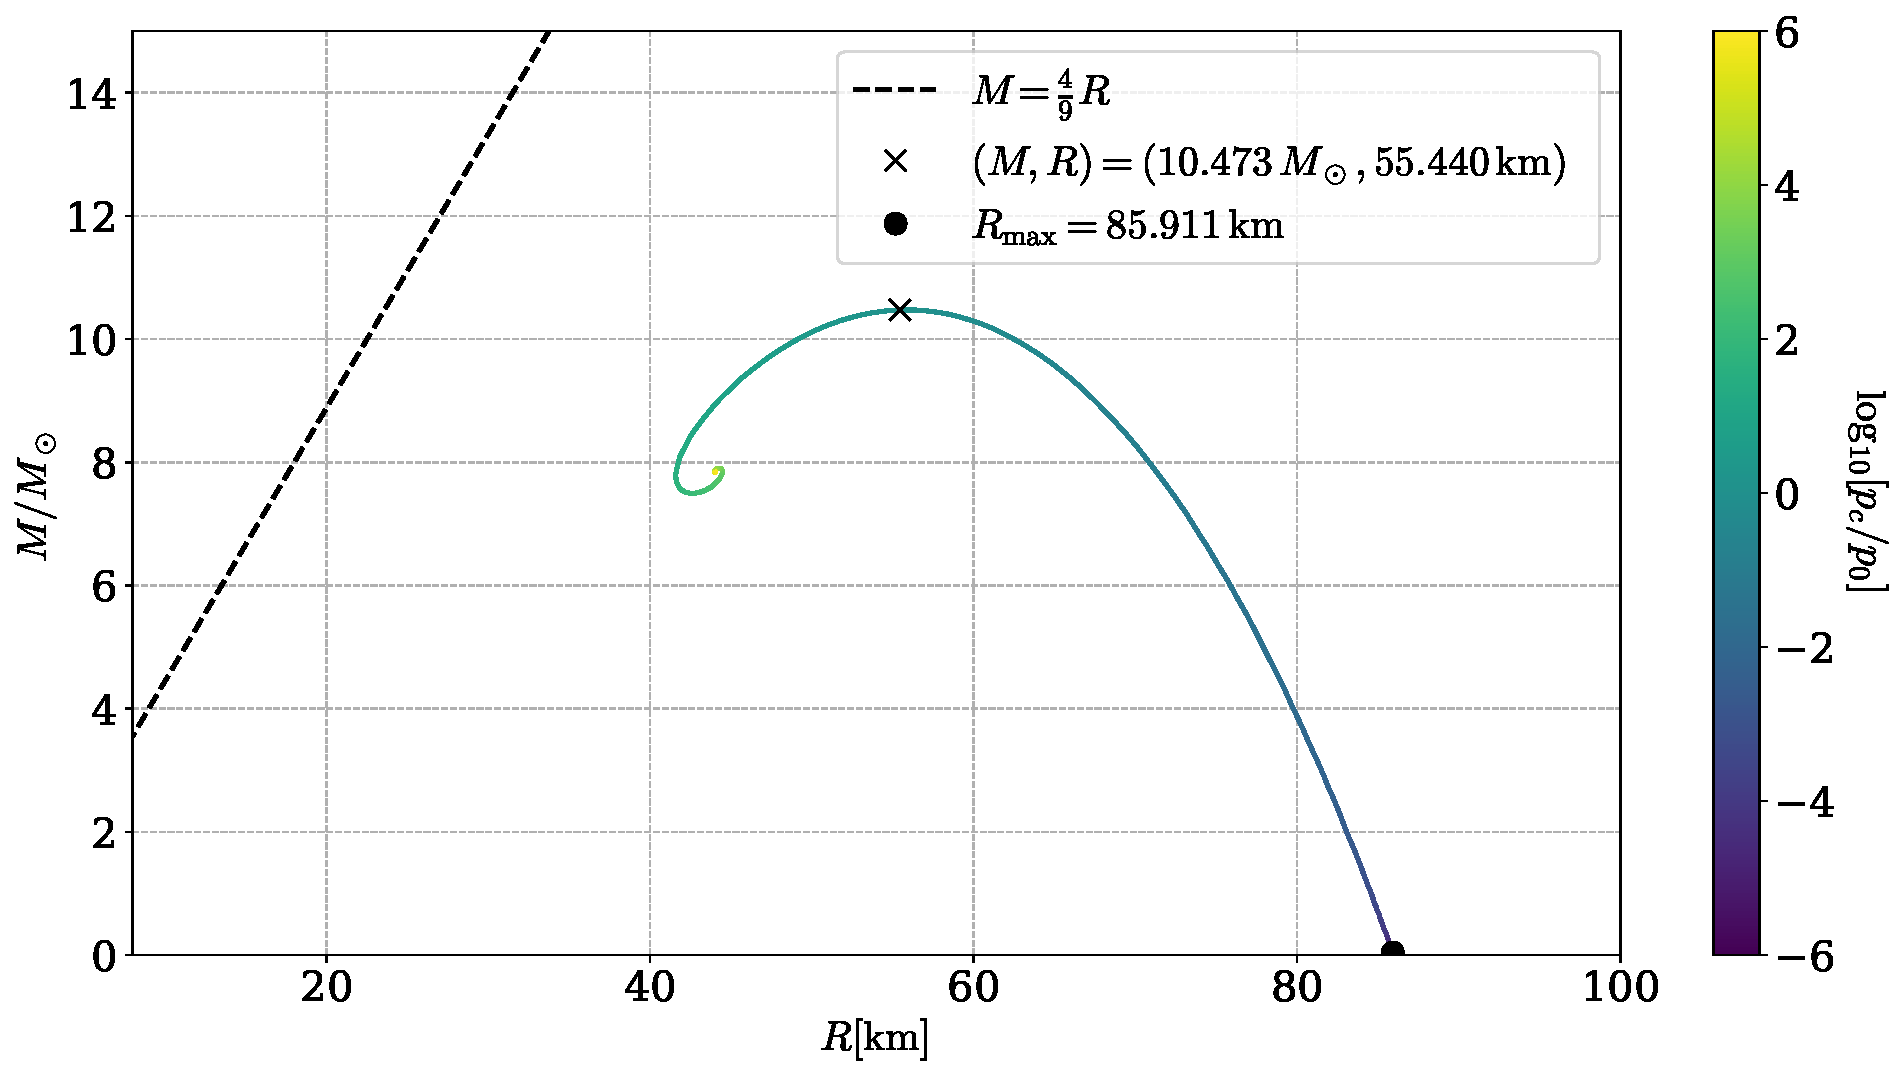
\includegraphics[width=0.85\textwidth]{../scripts/figurer/pion_star/mass_radius_pion_star.pdf}
    \caption{
        The plot shows the relationship between the mass and radius of a pion star. Mass is given in units of solar masses, while the radius is measured in kilometers.
        This line is parameterized by the central pressure $p_c$ of the star, as indicated by the color gradient.
        The dashed black line indicates the theoretical maximum mass for a given radius, and any configuration above it will collapse to a black hole.
        }
        \label{fig: mass-radius relation pion star}
\end{figure}

\begin{figure}[!h]
    \centering
    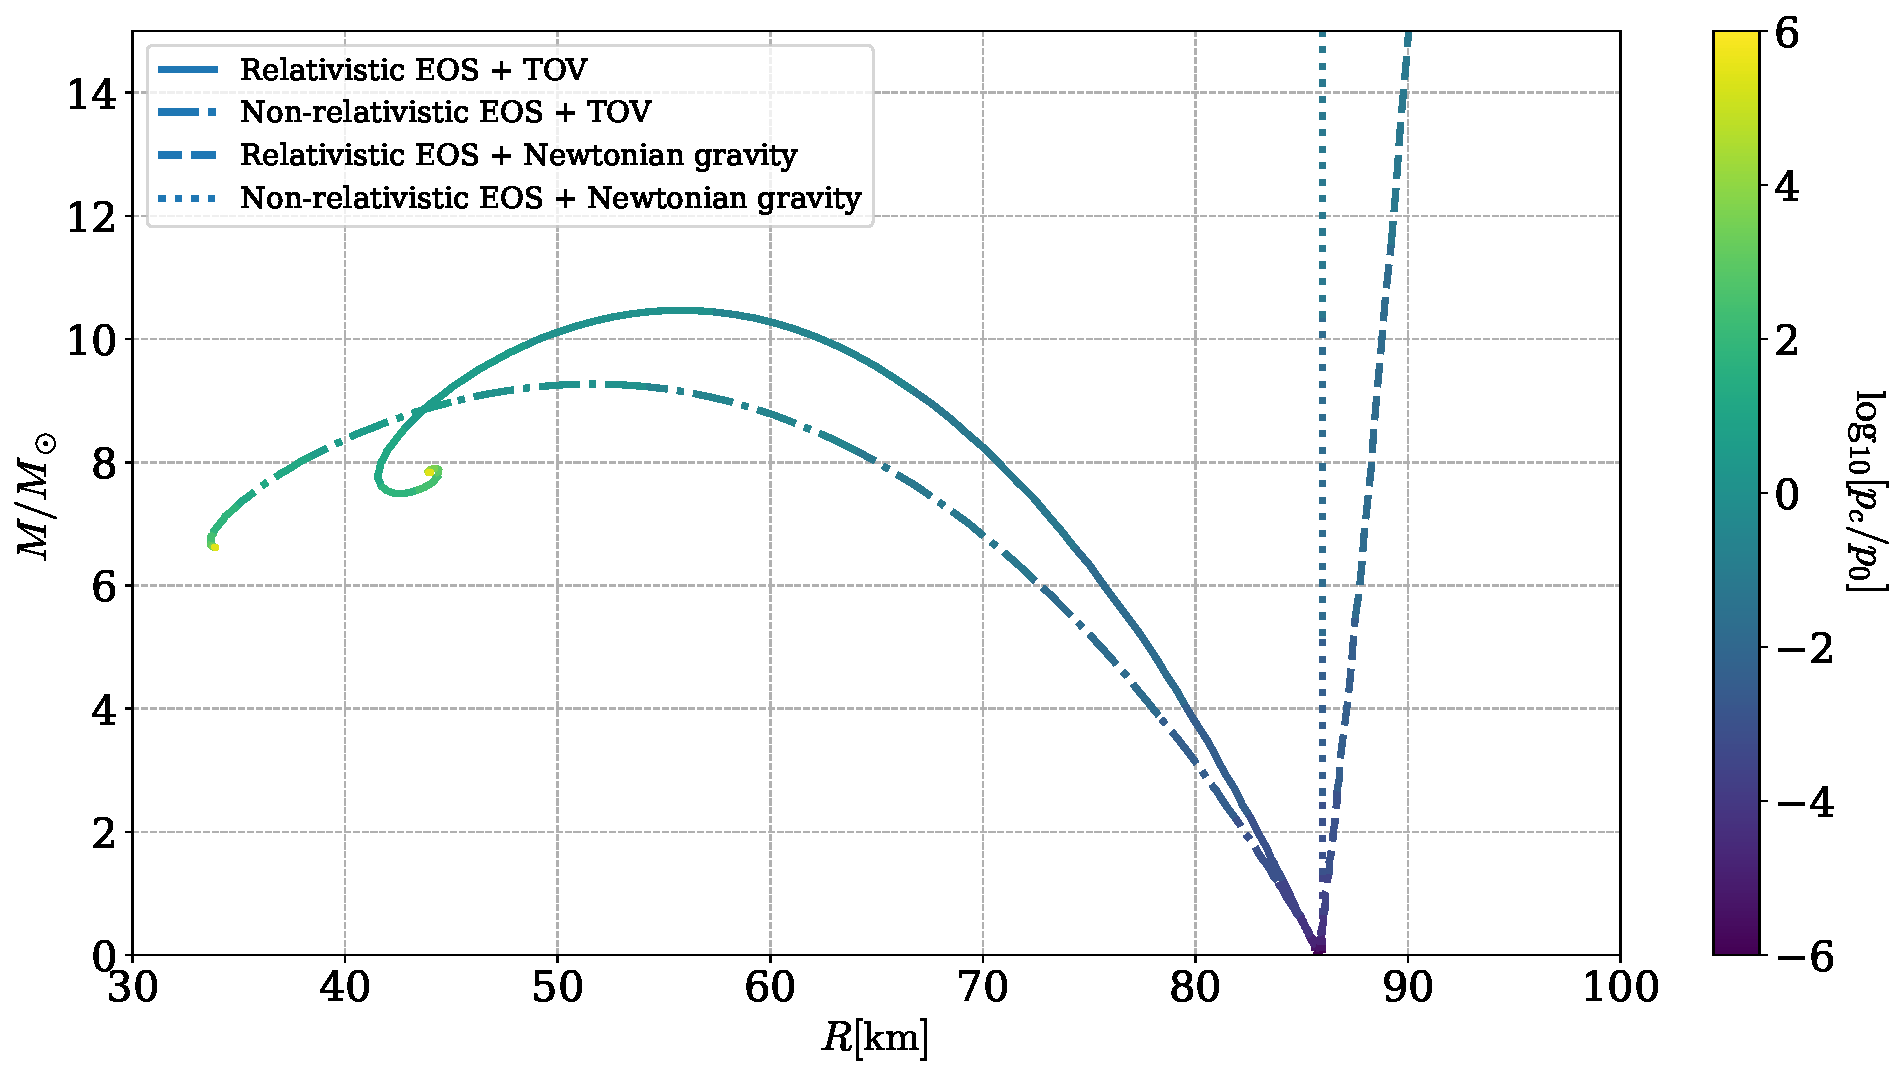
\includegraphics[width=0.85\textwidth]{../scripts/figurer/pion_star/mass_radius_comparison.pdf}
    \caption{
        The plot compares the mass-radius relationship of the pion star from the full equation of state and the TOV-equation with various limits.
        }
        \label{fig: mass-radius relation pion star comparison}
\end{figure}


\autoref{fig: mass-radius relation pion star} shows the mass-radius relation for the pion star.
As in the case of the neutron star, it has a maximum mass, in this case of $M_\text{max} = 10.47\, M_\odot$.
However, in contrast to the case of the neutron star, the stellar radius approaches a maximum radius as the central pressure decreases.
This matches our expectation from the non-relativistic, Newtonian limit.
We see that the largest radius in our results, corresponding to  $p_c = 10^{-6} \, p_0$, is $R = 85.82 \, \text{km}$, which is in good agreement with our earlier analysis, \autoref{radius pion star nr limit}.

\autoref{fig: mass-radius relation pion star comparison} compares the mass-radius relation from the full equation of state and TOV equation with various limits.
In the non-relativistic, Newtonian limit, the stellar radius is independent of the mass, as we found in our earlier analysis.

\todo[inline]{Vis kjemisk potensial}



\FloatBarrier
\subsection{Including electromagnetic contributions}

From \autoref{static lagrangian with EM}, the free energy density, including electromagnetic interactions, is
%
\begin{equation}
    \Eff =
    - f^2 \left[
        \bar m^2 \cos \alpha 
        + \frac{1}{2} \mu_I^2 \sin^2 \alpha
        + \frac{1}{2} \Delta m_\pm^2 \left(\cos^2 \alpha - \frac{4}{9}\right)
    \right].
\end{equation}
%
Free energy minimization now gives
%
\begin{equation}
    \frac{1}{u_0}\pdv{\Eff}{\alpha}
    = 
    \left[ \left( \frac{1}{x^2} - \Delta \right) \cos \alpha - 1\right] \sin \alpha = 0.
\end{equation}
%
Here, $x$ is defined as before, and we introduced the new quantity $\Delta = \Delta m_{\pm}^2 / \bar m^2= 0.06916$.
We see that the phase transition is raised, the critical chemical potential is now $\mu_I^c = \bar m \sqrt{1 + \Delta}$, the mass of the charged pions.
Below this value, $\alpha = 0$ remains the only solution.
In the pion condensate phase, the solution is
%
\begin{equation}
    \cos \alpha = \frac{x^2}{1 - \Delta x^2}.
\end{equation}
%
This reduces to our old solution for $\Delta = 0$, as it should.
With the same procedure as in the last section, we get the pressure and energy density
%
\begin{align}
    \tilde p_\text{EM} \
    & = \frac{1}{2} 
    \left[
        \frac{1}{x^2} 
        + \frac{x^2}{1 - x^2 \Delta} 
        - 2 - \Delta
    \right], \\
    \tilde u_\text{EM}
    &= \frac{1}{2} 
    \left[
        \frac{1}{x^2} 
        - x^2 \frac{3 - \Delta x^2}{(1 - \Delta x^2)^2}
        + 2 + \Delta)
    \right].
\end{align}
%

\begin{figure}[!htb]
    \centering
    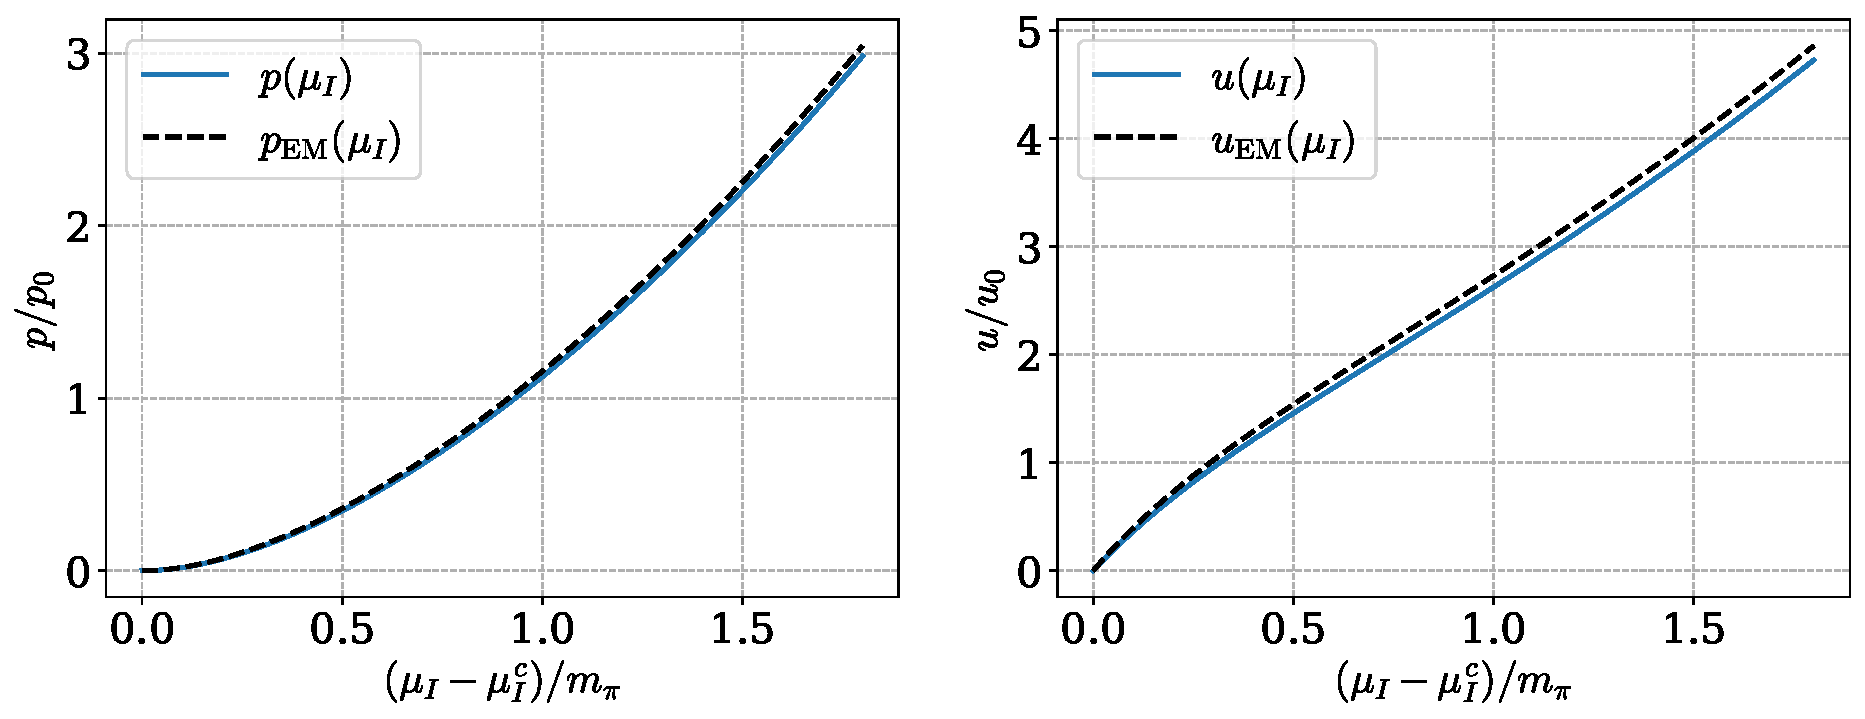
\includegraphics[width=0.95\textwidth]{../scripts/figurer/pion_star/pion_up.pdf}
    \caption{
        Left: The pressure, normalized to $p_0$, as a function of the chemical potential above the critical value, normalized to $\bar m$.
        Right: The energy density, normalized to $u_0$, also as a function of the chemical potential.
        Results with electromagnetic interaction are shown as dashed lines.
        }
        \label{fig: pressure and energy with EM interaction}
\end{figure}



\begin{figure}[!htb]
    \centering
    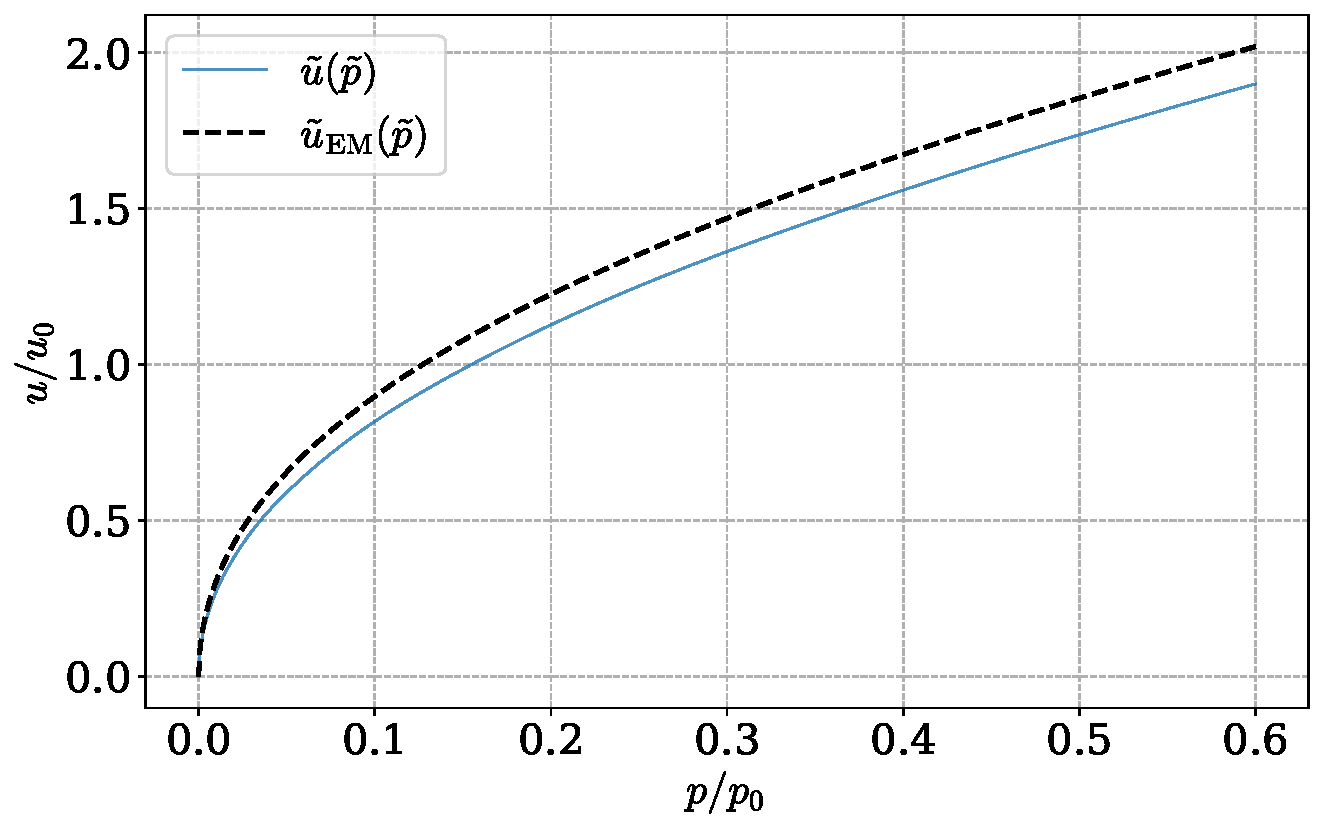
\includegraphics[width=0.65\textwidth]{../scripts/figurer/pion_star/pion_eos_EM.pdf}
    \caption{
        The equation of state in the pion condensate phase. 
        Results with electromagnetic interactions are shown as dashed lines.
        }
    \label{fig: eos chpt em interaction}
\end{figure}

In the limit $\Delta = 0$, these reduce to \autoref{pressure leading order chpt} and \autoref{energy density leading order chpt}.
In the ultra-relativistic limit, that is, for  $x \ll 1$, the behavior is the same as before, and we again approach $p = u$.
We find the non-relativistic limit by substituting $x^{-2} = 1 + \Delta + \epsilon$.
To first order in $\epsilon$ we get $\tilde p = \epsilon / 2$, which is the same as before.
However, the limit of the energy density is slightly perturbed by the inclusion of electromagnetism and is now $\tilde u = 2(1 + \Delta) \tilde \epsilon$.
The non-relativistic equation of state is thus still a polytrope of the form $p = K u^2$, however the constant is now $K^{-1} = 8 (1+\Delta)^2$.
With this, the radius of the polytrope and the limiting radius of the full system changes and is now
%
\begin{equation}
    R = \frac{\pi}{\sqrt{12}(1 + \Delta)} r_0 = 80.40 \, \text{km}.
\end{equation}


\autoref{fig: pressure and energy with EM interaction} shows the pressure and energy density, normalized to their characteristic quantities, as a function of chemical potential above the critical value, normalized to $\bar m$.
\autoref{fig: eos chpt em interaction} shows the equation of state.
The results with and without electromagnetic results are compared.

\autoref{fig: mass-radius relation leading order pion star with em interaction} shows the mass-radius reaction of the pion star when the electromagnetic interaction is taken into account.
We see that the shape of the curve has not changed much from our earlier result. 
Both the maximum mass and radius are slightly smaller. 
The result with and without electromagnetic interaction is compared in \autoref{fig: mass-radius relation comparison}.


\begin{figure}[!htb]
    \centering
    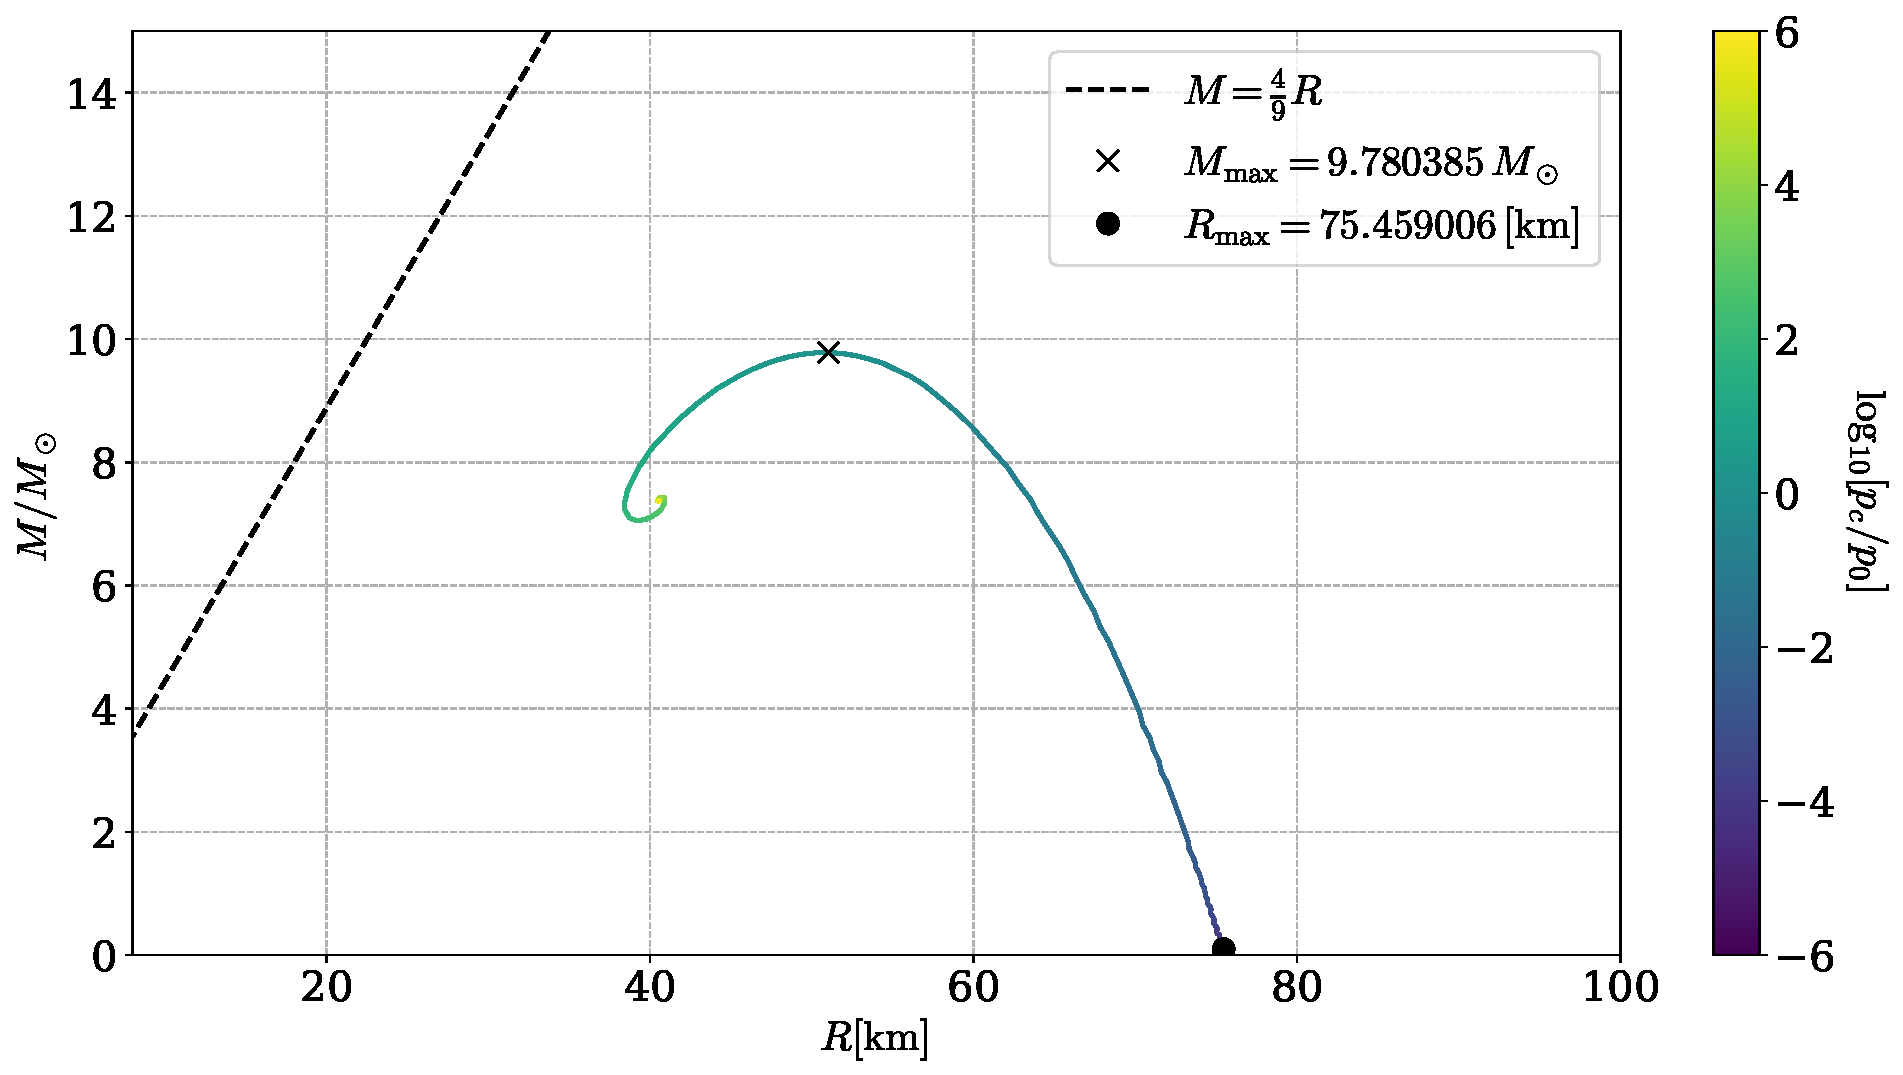
\includegraphics[width=0.85\textwidth]{../scripts/figurer/pion_star/mass_radius_pion_star_EM.pdf}
    \caption{
        The mass-radius relation of a pion star when the electromagnetic interactions is included. 
        The relation is parameterized by the logarithm of the central pressure. 
        The dashed line shows the absolute limiting mass for a given radius.
        The cross indicates the maximum mass configuration, and the dot the maximum radius configuration.
        }
    \label{fig: mass-radius relation leading order pion star with em interaction}
\end{figure}


\begin{figure}[!htb]
    \centering
    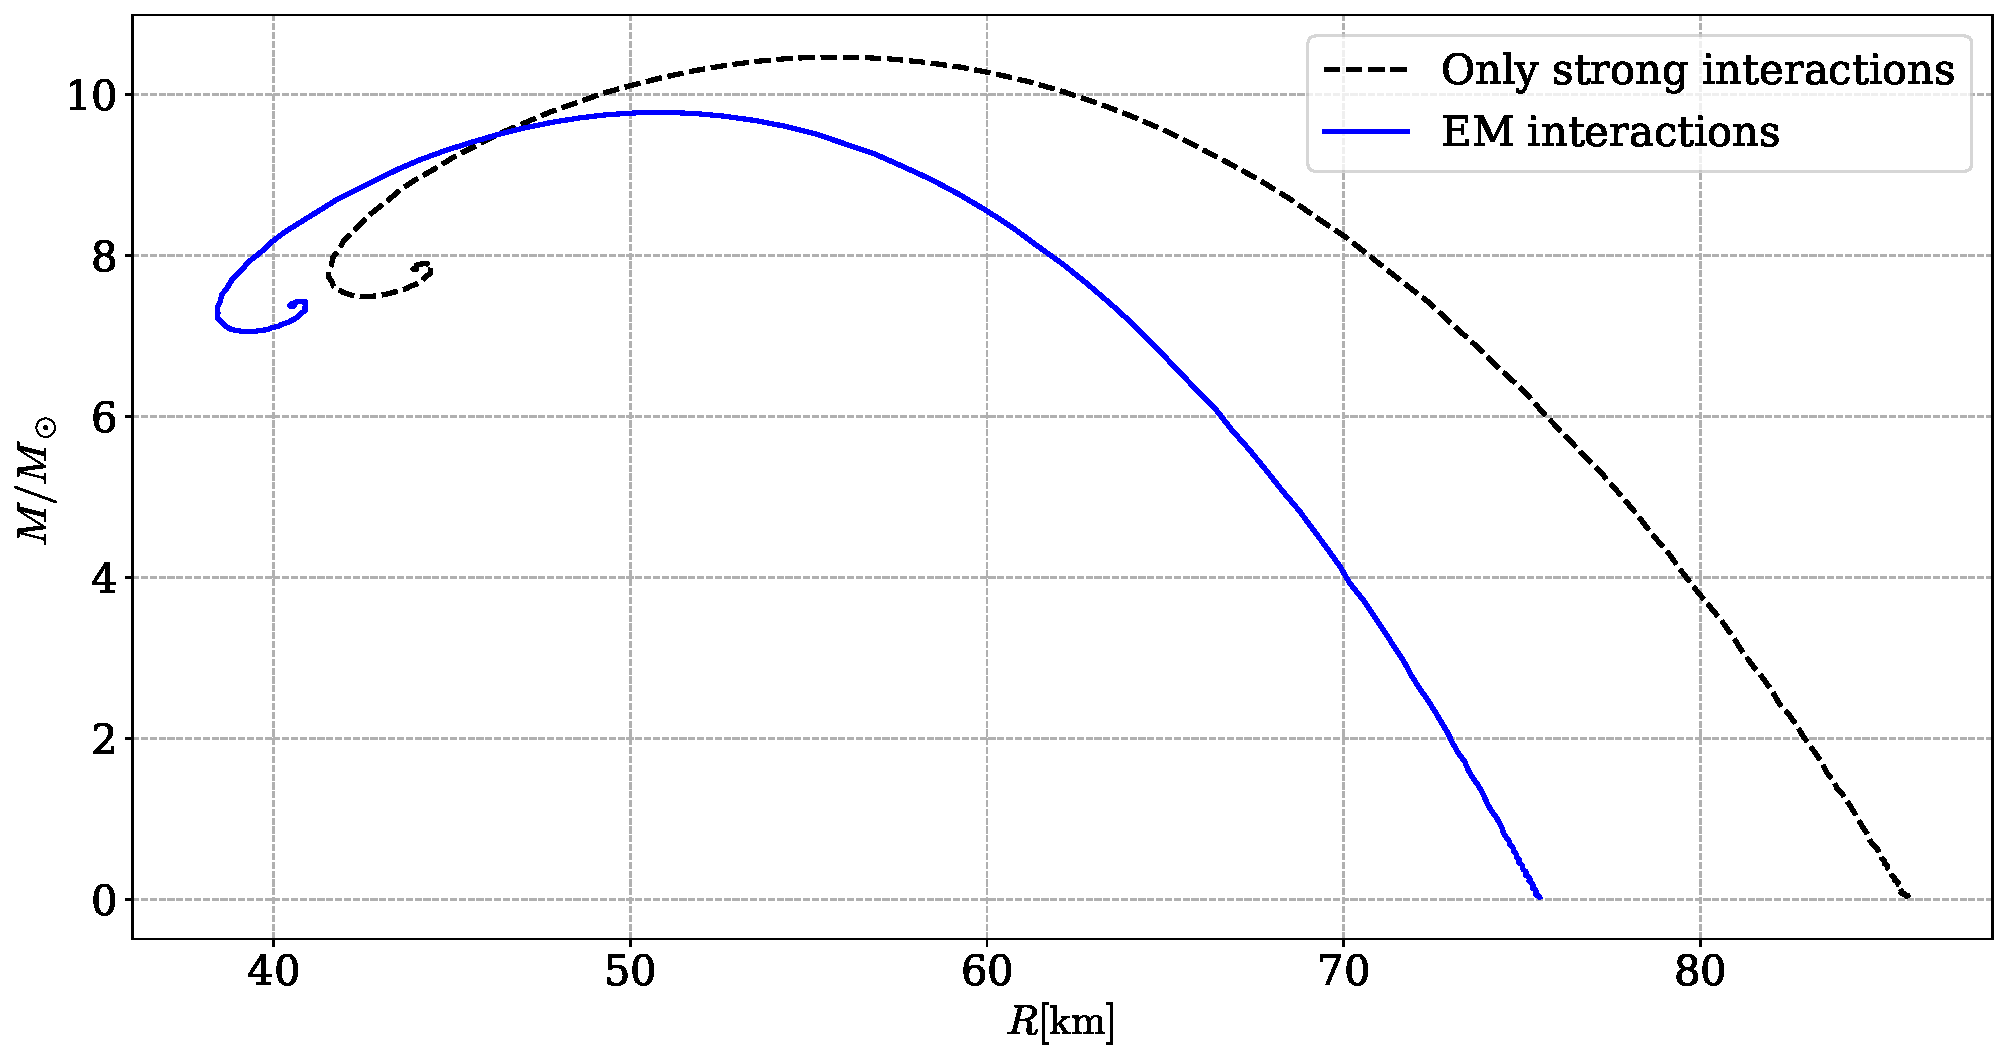
\includegraphics[width=0.85\textwidth]{../scripts/figurer/pion_star/mass_radius_pion_star_compare.pdf}
    \caption{
        This plot compares the mass-radius relation of pion stars with and without the inclusion of electromagnetism.
        }
        \label{fig: mass-radius relation comparison}
\end{figure}

